\documentclass[12pt,a4paper]{article}
\usepackage{ctex}
\usepackage{amsmath,amscd,amsbsy,amssymb,latexsym,url,bm,amsthm}
\usepackage{epsfig,graphicx,subfigure}
\usepackage{enumitem,balance}
\usepackage{wrapfig}
\usepackage{mathrsfs,euscript}
\usepackage[usenames]{xcolor}
\usepackage{hyperref}
\usepackage[vlined,ruled,linesnumbered]{algorithm2e}
\usepackage{array}
\usepackage[final]{pdfpages}
\hypersetup{colorlinks=true,linkcolor=black}

\newtheorem{theorem}{Theorem}
\newtheorem{lemma}[theorem]{Lemma}
\newtheorem{proposition}[theorem]{Proposition}
\newtheorem{corollary}[theorem]{Corollary}
\newtheorem{exercise}{Exercise}
\newtheorem*{solution}{Solution}
\newtheorem{definition}{Definition}
\theoremstyle{definition}

\renewcommand{\thefootnote}{\fnsymbol{footnote}}

\newcommand{\postscript}[2]
 {\setlength{\epsfxsize}{#2\hsize}
  \centerline{\epsfbox{#1}}}

\renewcommand{\baselinestretch}{1.0}

\setlength{\oddsidemargin}{-0.365in}
\setlength{\evensidemargin}{-0.365in}
\setlength{\topmargin}{-0.3in}
\setlength{\headheight}{0in}
\setlength{\headsep}{0in}
\setlength{\textheight}{10.1in}
\setlength{\textwidth}{7in}
\makeatletter \renewenvironment{proof}[1][Proof] {\par\pushQED{\qed}\normalfont\topsep6\p@\@plus6\p@\relax\trivlist\item[\hskip\labelsep\bfseries#1\@addpunct{.}]\ignorespaces}{\popQED\endtrivlist\@endpefalse} \makeatother
\makeatletter
\renewenvironment{solution}[1][Solution] {\par\pushQED{\qed}\normalfont\topsep6\p@\@plus6\p@\relax\trivlist\item[\hskip\labelsep\bfseries#1\@addpunct{.}]\ignorespaces}{\popQED\endtrivlist\@endpefalse} \makeatother

\begin{document}
\noindent

%========================================================================
\noindent\framebox[\linewidth]{\shortstack[c]{
\Large{\textbf{Lab09-Network Flow}}\vspace{1mm}\\
CS214-Algorithm and Complexity, Xiaofeng Gao, Spring 2020.}}
\begin{center}
\footnotesize{\color{red}$*$ If there is any problem, please contact TA Shuodian Yu. }

\footnotesize{\color{blue}$*$ Name:Haotian Xue  \quad Student ID:518021910506 \quad Email: xavihart@sjtu.edu.cn}
\end{center}
\begin{enumerate}
\item Given a weighted directed graph $G(V, E)$ and its corresponding weight matrix $W=(w_{ij})_{n \times n}$ and shortest path matrix $D=(d_{ij})_{n \times n}$, where $w_{ij}$ is the weight of edge $(v_i, v_j)$ and $d_{ij}$ is the weight of a shortest path from pairwise vertex $v_i$ to $v_j$. Now, assume the weight of a particular edge $(v_a, v_b)$ is decreased from $w_{ab}$ to $w'_{ab}$. Design an algorithm to update matrix $D$ with respect to this change, whose time complexity should be no larger than $O(n^2)$. Describe your design first and write down your algorithm in the form of pseudo-code.
    \begin{solution}
		Since the shortest path between any two vertices before the modification are given, then for any two vertices $x$ and $y$, if the shortest path between this two vertices includes $(v_a, v_b)$, $d(x, y)$ should be modified.
	The above situation will happen if and only if $d(x, y) = d(x, v_a) + d(v_b, y)$ or $d(x, y) = d(x, v_b) + d(v_a, y)$. So we can use two loops to tranverse all the $(x, y)$ pairs and try to renew the shortest path.
	Then time complexity is obvious no larger than $O(n^2)$. The pseudo code is as follows:
	
	\begin{minipage}[t]{0.90\textwidth}
		\begin{algorithm}[H]
			%\algsetup{footnotesize}
			%\scriptsize
			\KwIn{$G(V,E)$, $D = (d_{ij})_{n\times n}$.}
			\KwOut{updated $D$}
			
			$D^{'} = D = (d^{'}_{ij})_{n\times n}$

	
	
			\For{$x$ in $V$}{
				\For{$y$ in $V$}{
					\If{$d^{'}_{xy} = d^{'}_{{xv}_a} + w_{ab} + d^{'}_{{v_b y}}$}{
                         $d_{xy} = d^{'}_{{xv}_a} + w^{'}_{ab} + d^{'}_{{v_b y}}$    
					}

					\If{$d^{'}_{xy} = d^{'}_{{xv}_b} + w_{ab} + d^{'}_{{v_a y}}$}{
                         $d_{xy} = d^{'}_{{xv}_b} + w^{'}_{ab} + d^{'}_{{v_a y}}$    
					}

				}
			}
		
			\Return{$D$}\;
			
		\end{algorithm}
	\end{minipage}
    \end{solution}

	\item Given a directed graph $G$, whose vertices and edges information are introduced in data file ``SCC.in''. Please find its number of Strongly Connected Components with respect to the following subquestions.
    \begin{enumerate}
    	\item Read the code and explanations of the provided C/C++ source code ``SCC.cpp'', and try to complete this implementation.
    	\item Visualize the above selected Strongly Connected Components for this graph $G$. Use the $Gephi$ or other software you preferred to draw the graph. {\color{blue}(If you feel that the data provided in ``SCC.in'' is not beautiful, you can also generate your own data with more vertices and edges than $G$ and draw an additional graph. Notice that results of your visualization will be taken into the consideration of Best Lab.)}

    \end{enumerate}
    \begin{solution}
		(a) Tarjan algorithm is used to solve the SCC problem, and the code is in $./SCC.cpp$ and the result for the test case id $666$.
		
		(b) To visualize the $100000$ vertices, I do some modifications according to results in (a). To be specific, the Strongly Connected Components are treated as new vertices in the generated graph $G^{'} = (V^{'}, E^{'})$ and for any two SCC $SCC_1$ and $SCC_2$, we have:

		\begin{equation*}
			(SCC_1, SCC) \in E^{'}  \Leftrightarrow \exists v_1 \in SCC_1 ~ , v_2 \in SCC_2 ~ st. (v_1, v_2) \in E
		\end{equation*}
	  

		according to the results in (a), we have $|V^{'}| = 666$, the visualization is generated by Gephi with certain distribution and the color of nodes are determined by their ranks. The figures can be referred to in the last page 
		of this lab report.
		

		
	\end{solution}
	\item The \textbf{Minimum Cost Maximum Flow} problem (MCMF) is an optimization problem to find the cheapest possible way of sending the maximum amount of flow through a flow network. That is, in a flow network $G = (V, E)$ with a source $s\in V$ and a sink $t\in V$, where each edge $(u, v)\in E$ has a capacity $c(u,v) > 0$ and a cost $a(u,v) \ge 0$, find a maximum $s\text{-}t$ flow $f$ over all edges ($f(u, v) \ge 0)$, such that the total cost of $\sum_{(u, v) \in E} a(u, v) \cdot f(u, v)$ is minimized.

A common greedy approach to solve the MCMF problem can be described as follows: We can modify Ford-Fulkerson algorithm, where each time we choose the least cost path from $s$ to $t$. To do this correctly, when we add a back-edge to some edge $e$ into the residual graph, we give it a cost of $-a(e)$, representing that we get our money back if we undo the flow on it.

Note that such procedure may create a residual graph with negative-weight edges, which is not suitable for Dijkstra's Algorithm. However, motivated by Johnson's Algorithm, we can reweight the edge cost with vertex labels and convert the weight non-negative again.

Please prove the correctness of such greedy approach and implement this algorithm in C/C++. The file \emph{MCMF.in} is a test case, where the first line contains four graph parameters $n$, $m$, $s$, $t$, and the rest $m$ lines exhibit the information of $m$ edges. Each line contains four integers: $u_i$, $v_i$, $c_i$, $a_i$, denoting that there is an edge from $u_i$ to $v_i$ with capacity $c_i$ and cost $a_i$. {\color{blue}(Your source code should be named as \emph{MCMF.cpp} and output the maximum flow and minimum cost of this test case.)}

\fbox{
\begin{minipage}[t]{0.2\textwidth}
\textbf{Sample Input:}
	
	4 5 4 3 \\ 4 2 30 2 \\ 4 3 20 3 \\ 2 3 20 1 \\ 2 1 30 9 \\ 1 3 40 5
\end{minipage}
\begin{minipage}[t]{0.2\textwidth}
\textbf{Sample Output: }
	
	50 280
\end{minipage}}
\hspace{1cm}
\begin{minipage}[t]{0.45\textwidth}
\textbf{Remark:} The source code \emph{SCC.cpp}, and the input data \emph{SCC.in} and \emph{MCMF.in} are attached on the course webpage. Please include your .pdf, .tex, .cpp files for uploading with standard file names.
\end{minipage}
    \begin{proof}
		 The code is in $./MCMF.cpp$ and with the input in $./MCMF.in$ and output in $./MCMF.out$. We call ResGraph as short for the residual graph. 

	\textbf{Brief description:} In each iteration, we figure out the path with the least cost in the ResGraph and increase the flow in the path by the bottleneck flow. Then we keep doing this until there is no
	path between $s$ and $t$ in the ResGraph. Then let's proof the correctness of this algorithm for finding the MCMF.

	
	\begin{lemma}
		For flow $f$, $f$ is the minimal cost flow $\Leftrightarrow$ there exists no cycle with negative cost.
	\end{lemma}
	
	\begin{proof}
		"$\Rightarrow$":
		Suppose there is a negative-cost cycle in the ResGraph, it is $v_1 -> v_2 -> ... -> v_k$, and the edges in the cycle is: $e_1 = (f_1, c_1), ..., e_k = (f_k, c_k)$, 
		where $f_i$ and $c_i$ are the flow and cost respectively. Then we agument the flow along the negative cycle, that will obviously not affect the property of flows. Since for every edge 
		agumented, the in-flow changes with respect to the out-flows. 
		
		The most import thing we want to know is that the operation above will destroy the negative cycles in finite steps. 
		Think about $e_1, e_2, ..., e_k$, after each iteration of agumentation of cycle, the $f_1, f_2, ..., f_k$ is decreasing and it is sure that after finite steps, some of them will become 
		zero, which make the negative cycle destroied. 

		Also, we can proof the operation will decrease the cost of flow. The key point is: the cost of a flow edge(inversed edge) in a ResGraph is always negtive. So for the negative
		cycle, we have the change of total cost:

		\begin{equation*}
			\Delta{\sum_{e}{f(e)c(e)}} = min(f_1, ..., f_k) * \sum_{i=1}^{k}c_i 
		\end{equation*}

		Since in the negative cycle, we have $\sum_{i=1}^{k}c_i < 0$, then we can see the total cost is decreasing.

		So we can proof the lemma by contradiction, there is no negative cycle in the ResGraph of MCMF actually. 
	
		"$\Leftarrow$": If there exits one flow $f^{'}$ which has a cost fewer than $f$, we think about $f^{'} - f$, which is made up of cycles and since $f^{'}$ has a fewer cost than $f$. 
		We can see $f{'} - f$ must has negative cycles in it, which makes sense in the ResGraph of $f$ as well since the 
		
		\begin{lemma}
	  During the algorithm, no negative cycle is generated.
		
		\end{lemma}


		\begin{proof}
			If we generate one negative cycle $C$ contains$v_1, v_2, ..., v_k$. Since the edges on the new path $P$ has a negative cost, and we have $c < 0$ is the sum of cost of $P \cap C$.
			so the sum of cost on rest edges must be smaller than $|q|$. So if we change $P$ to $C - P$, the cost will be fewer, wihch contradicts with the shortest path. 
		\end{proof}

	\end{proof}
   		Considering the above two lemmas, we can get that the algorithm is correct.	


    \end{proof}


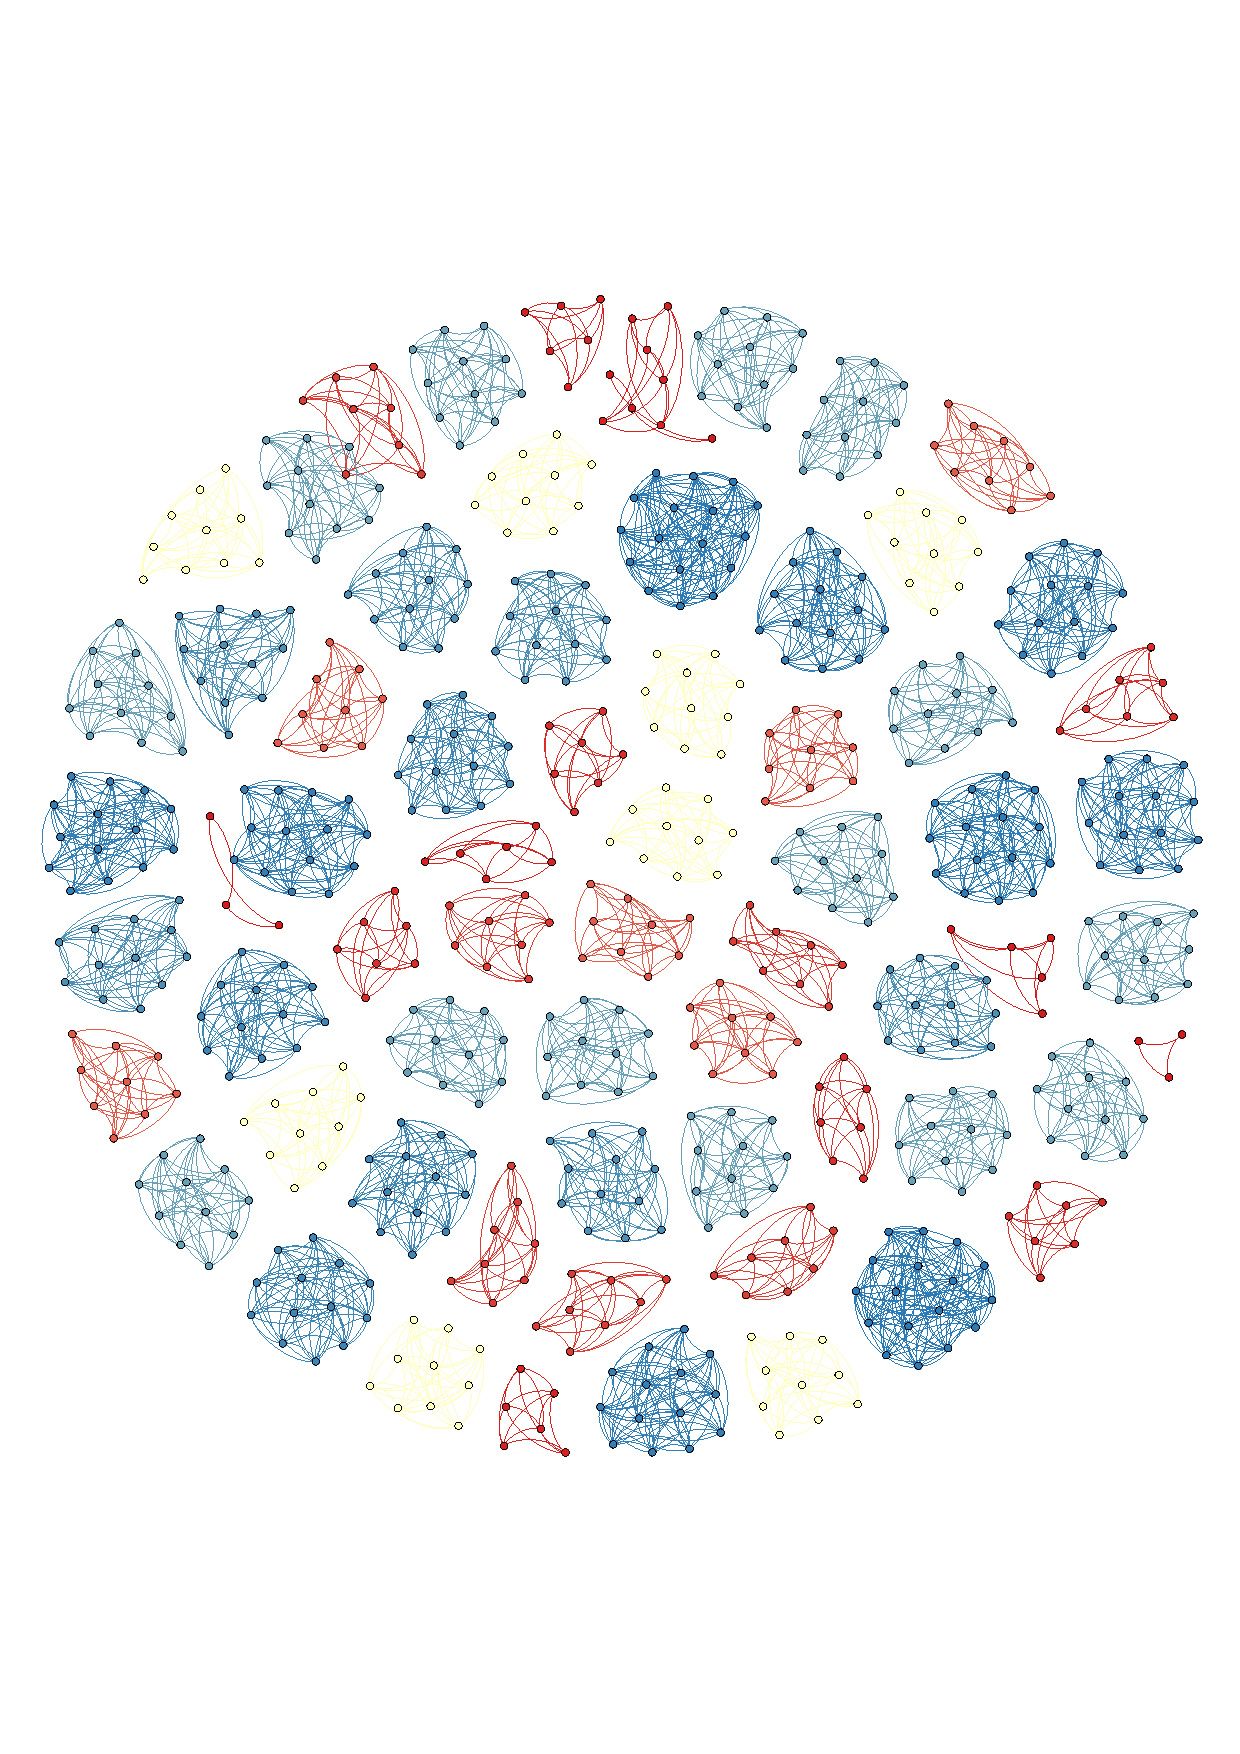
\includepdf{./P2.pdf} 
\newpage
\end{enumerate}






%========================================================================
\end{document}
